\documentclass[a4paper]{article}

\usepackage[utf8]{inputenc}
\usepackage[spanish]{babel}
\usepackage[margin=2cm, top=2cm, includefoot]{geometry}%--para definir espacio de márgenes
\usepackage{graphicx}%--para insertar imágenes
\usepackage{fancyhdr}%--para el estilo con barra arriba de las páginas
\usepackage[table,xcdraw]{xcolor}%--para la detección de colores
\usepackage[hidelinks]{hyperref}%--para hipervínculos
\usepackage{parskip}%--para evitar tabulación de inicio de párrafo
\usepackage{booktabs}%--
\usepackage{multirow, array}
\usepackage{ragged2e}
\usepackage{float}

%definiendo color
\definecolor{rojoOscuro}{HTML}{A20303}
%---definiendo estilo del informe
\setlength{\headheight}{47pt}
\pagestyle{fancy}
\fancyhf{}
\lhead{\hspace{0.1cm} 
\includegraphics[height=1.55cm]{imagenes/CiberSecFIIS.png}}\rhead{
\includegraphics[height=1.5cm]{imagenes/uni_logo.png} \hspace{0.1cm}}

%---Cambios
\renewcommand{\headrulewidth}{3pt}%--grosor de la linea superior
\renewcommand{\headrule}{\hbox to\headwidth{\color{rojoOscuro}\leaders\hrule height \headrulewidth\hfill}}%--definir la linea base superior
\renewcommand{\arraystretch}{2}%--espaciado de las tablas
%---Inicio de informe
\begin{document}
    \begin{titlepage}
    \centering
        {\large \textbf{UNIVERSIDAD NACIONAL DE INGENIERÍA}} \par \vspace{0.3cm}
        {\large \textbf{FACULTAD DE INGENIERÍA INDUSTRIAL Y DE SISTEMAS}} \par \vspace{1.125cm}
        
\includegraphics[width=0.7\textwidth]{imagenes/CiberSecFIIS.png} \par \vspace{1.125cm}
        {\LARGE \textbf{Segunda Evaluación de Penetración de Seguridad}}\par \vspace{1cm}
        {\Large \textbf{Elaborado por:}} \par \vspace{1cm}
        {\large \textbf{Elian Paucar}} \par \vspace{0.8cm}
        {\large \textbf{Rodrigo Rojas}} \par \vspace{0.8cm}
        {\large \textbf{Sandro Castillo}} \par \vspace{2.75cm}
        \vfill
        {\textbf{Lima, 2021}}
\end{titlepage}
%-----------------------------------------------------------
    \clearpage
        \tableofcontents
    \clearpage
%------------------------------------------------------------
    \listoffigures
    \clearpage
%------------------------------------------------
    %----Para el inicio de numeración a partir de aquí---
    \cfoot{\thepage}
    \setcounter{page}{1}
 %--------Resumen ejecutivo------------
 \addcontentsline{toc}{section}{Resumen Ejecutivo} %--Para que sección sin numeración aparezca en el índice
    \begin{center}
        \section*{Resumen Ejecutivo}
    \end{center}
\vspace{0.1cm}
\begin{large}
\justify{
El presente informe contiene todas las acciones realizadas por miembros del grupo CibersecFIIS para realizar una evaluación de seguridad y pruebas de penetración a cuatro computadoras pertenecientes a la plataforma Hack The Box.
\\
El propósito de este informe es evaluar y mejorar los conocimientos en ciberseguridad del equipo auditor haciendo uso de la plataforma Hack The Box.
\\
El actual informe detalla el alcance de las pruebas realizadas y los hallazgos importantes junto con las recomendaciones para mitigar vulnerabilidades. A continuación, se proporciona un resumen de los hallazgos clave descubiertos durante la evaluación.
\\
La cantidad de vulnerabilidades encontradas por máquina se resume en el siguiente gráfico.
}
\end{large}
\begin{figure}[h]
    \centering
    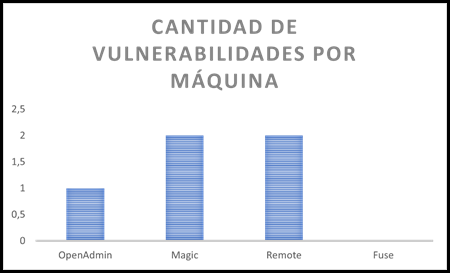
\includegraphics[width=0.7\textwidth]{imagenes/vuln_x_maq.png}
    \caption{Cantidad de vulnerabilidades por máquina}
\end{figure}

\large{El total de vulnerabilidades encontradas según su tipología se distribuyen de la siguiente forma:}
\\
\begin{figure}[h]
    \centering
    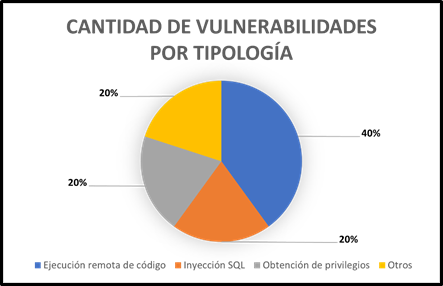
\includegraphics[width=0.7\textwidth]{imagenes/vuln_x_tipo.png}
    \caption{Cantidad de vulnerabilidades por tipología}
\end{figure}
\\
\large{De las 5 vulnerabilidades, solo 2 tienen identificador CVE asociado.}
\\
\\
\large{La cantidad de debilidades encontradas por máquina durante las pruebas de penetración se resume de la siguiente forma.}
\begin{figure}[h]
    \centering
    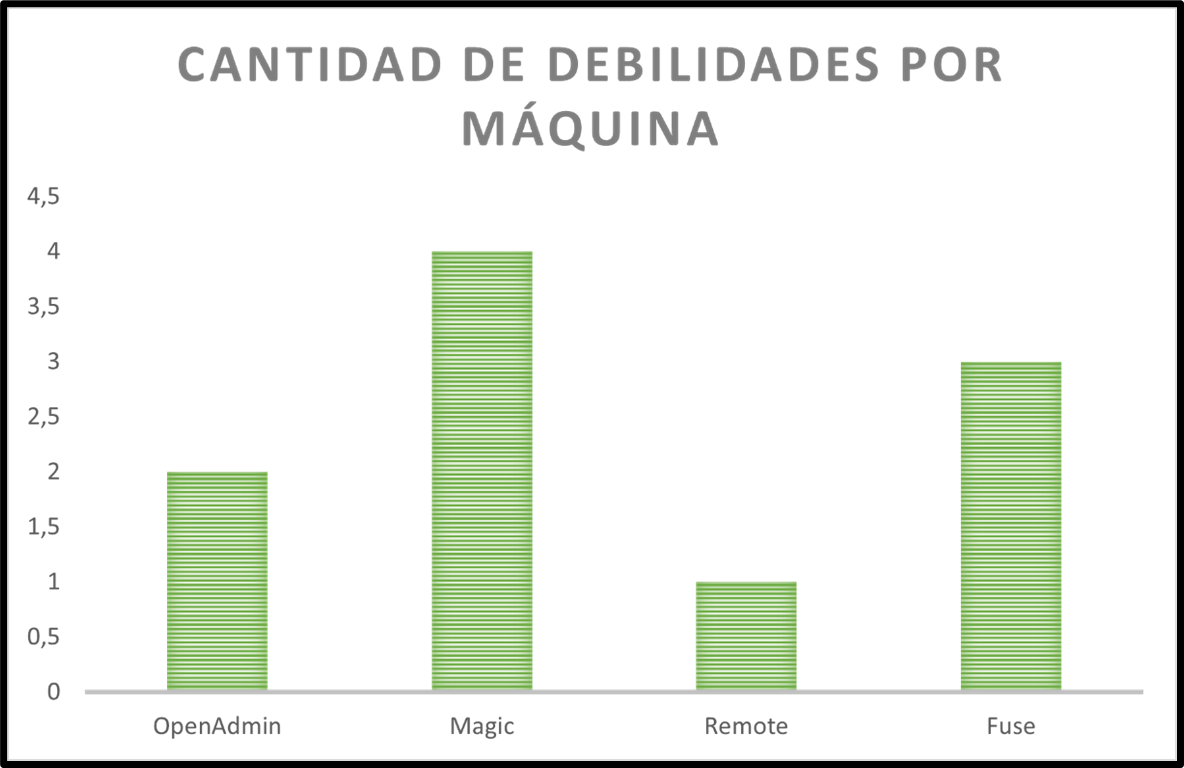
\includegraphics[width=0.7\textwidth]{imagenes/deb_x_maq.png}
    \caption{Cantidad de debilidades por máquina}
\end{figure}
\\
\large{La cantidad de máquinas relacionadas a un tipo de debilidad se distribuyen en el siguiente gráfico.}
\\
\begin{figure}[h]
    \centering
    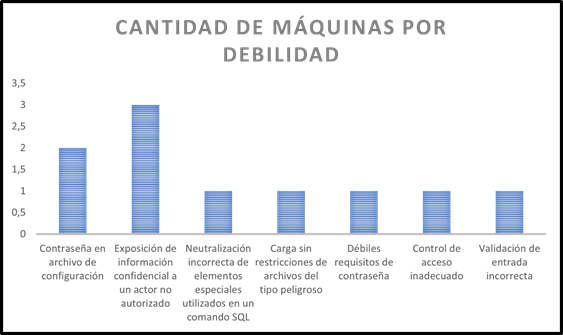
\includegraphics[width=0.7\textwidth]{imagenes/maq_x_deb.png}
    \caption{Cantidad de máquinas por debilidad}
\end{figure}
\\
\large{Según la cantidad de vulnerabilidades y debilidades en cada máquina, se puede observar que la máquina “Magic” es la más insegura con 2 vulnerabilidades y 4 debilidades.}

%-------------------------------------------------
\clearpage
\section{Objetivo}
\large{El objetivo de la presente evaluación de penetración de seguridad es encontrar vulnerabilidades y hacer una evaluación de criticidad de estas con el fin de que el negocio no se vea afectado por algún ataque malicioso que pueda afectar la calidad de sus servicios y su imagen.}
\par
\section{Alcance}
\large{El alcance de esta evaluación se limita a las pruebas en los computadores de la plataforma Hack The Box con las siguientes direcciones IP:}
\par
\begin{table}[h]
    \centering
    \begin{tabular}{|c|c|c|c|c|} \hline
        Identificador & Nombre de host & Dirección IP & Sistema Operativo & Dificultad \\ \hline
        HTB01 & OpenAdmin & 10.10.10.171 & Linux & Fácil \\ \hline
        HTB02 & Magic & 10.10.10.185 & Linux & Medio \\ \hline
        HTB03 & Remote & 10.10.10.180 & Windows & Fácil \\ \hline
        HTB04 & Fuse & 10.10.10.193 & Windows & Medio \\ \hline
    \end{tabular}
    \caption{Datos sobre las máquinas}
\end{table}
\par
\section{Detalle de Hallazgos}
\large{Los hallazgos encontrados en la evaluación de penetración de seguridad fueron los siguientes:}
\par
\vspace{0.1cm}
Se encontraron 5 vulnerabilidades, pertenecientes a 3 de 4 máquinas.
\par
\begin{table}[h]
    \centering
    \begin{tabular}{|c|c|m{2.9cm}|c|c|c|c|c|} \hline
        Identificador & CVE & \centering{Tipo de vulnerabilidad} & CVSSv2 & OpenAdmin & Magic & Remote & Fuse \\ \hline
        VU01 & - & \centering{Ejecución Remota de Código} & - & \Large{\begin{math}\bullet\end{math}} &  &  &  \\ \hline
        VU02 & - & \centering{Inyección SQL} & - &  & \Large{\begin{math}\bullet\end{math}} &  &  \\ \hline
        VU03 & CVE-2017-6516 & \centering{Obtención de privilegios} & 7.2 &  & \Large{\begin{math}\bullet\end{math}} &  &  \\ \hline
        VU04 & - & \centering{Ejecución Remota de Código} & - &  &  & \Large{\begin{math}\bullet\end{math}} &  \\ \hline
        VU05 & CVE-2019-1322 & \centering{Otros} & 4.6 &  &  & \Large{\begin{math}\bullet\end{math}} &  \\ \hline
    \end{tabular}
    \caption{Vulnerabilidades encontradas}
\end{table}

\clearpage
Se encontraron 7 debilidades entre las 4 máquinas objetivo.
\par
\begin{table}[h]
    \centering{
    \begin{tabular}{|c|c|m{4.5cm}|c|c|c|c|} \hline
        Identificador & CWE & \centering{Debilidad} &  OpenAdmin & Magic & Remote & Fuse \\ \hline
        DE01 & CWE-260 & \centering{Contraseña en archivo de configuración} & \Large{\begin{math}\bullet\end{math}} & \Large{\begin{math}\bullet\end{math}} &  &  \\ \hline
        DE02 & CWE-200 & \centering{Exposición de información confidencial a un actor no autorizado} & \Large{\begin{math}\bullet\end{math}} & & \Large{\begin{math}\bullet\end{math}} & \Large{\begin{math}\bullet\end{math}} \\ \hline
        DE03 & CWE-89 & \centering{Neutralización incorrecta de elementos especiales utilizados en un comando SQL} &  & \Large{\begin{math}\bullet\end{math}} &  &  \\ \hline
        DE04 & CWE-434 & \centering{Carga sin restricciones de archivos del tipo peligroso} & & \Large{\begin{math}\bullet\end{math}} & &  \\ \hline
        DE05 & CWE-521 & \centering{Débiles requisitos de contraseña} & & & & \Large{\begin{math}\bullet\end{math}} \\ \hline
        DE06 & CWE-284 & \centering{Control de acceso inadecuado} & & & & \Large{\begin{math}\bullet\end{math}} \\ \hline
        DE07 & CWE-20 & \centering{Validación de entrada incorrecta} & & \Large{\begin{math}\bullet\end{math}} & & \\ \hline
    \end{tabular}
    \caption{Vulnerabilidades encontradas}}
\end{table}
\par
Los tipos de vulnerabilidades reconocidas son extraídos de la página CVE Details \cite{cvedetails}. 

\vspace{0.1cm}
Los puntajes CVSS v2 fueron extraídos de la página Vulmon – Vulnerability Intelligence Search Engine \cite{vulmon}.

\vspace{0.1cm}
La información relacionada a los tipos de debilidades es extraída de la página Common Weakness Enumeration de MITRE \cite{cwe}.
%-----------Empieza pruebas de penetración----------
\clearpage
    \section{Desarrollo de pruebas de penetración}
\subsection{HTB01 - OpenAdmin}
\subsubsection{Escaneo}
Como inicio de la prueba de penetración se realiza un escaneo de puertos con la herramienta “Nmap”, donde se encuentran dos puertos abiertos, el puerto 22 con el servicio SSH y el puerto 80 con un servidor web Apache.
\begin{figure}[H]
    \centering
    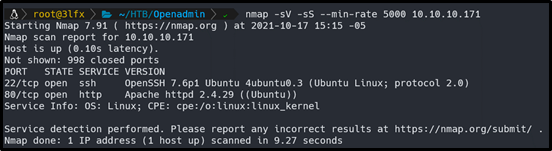
\includegraphics[width=0.99\textwidth]{imagenes/scanopen.png}
    \caption{Escaneo de puertos OpenAdmin}
\end{figure}
\subsubsection{Análisis de vulnerabilidades y debilidades}
Se procedió a revisar el sitio web, teniendo la solo la página predeterminada de Apache.
\begin{figure}[H]
    \centering
    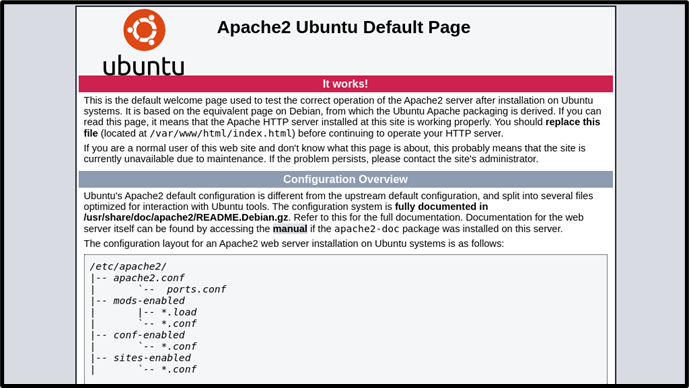
\includegraphics[width=0.99\textwidth]{imagenes/apapred.png}
    \caption{Página web predeterminada de Apache en OpenAdmin}
\end{figure}
Lo siguiente a realizar fue usar la herramienta “Gobuster” para enumerar los directorios del servidor web.

\begin{figure}[H]
    \centering
    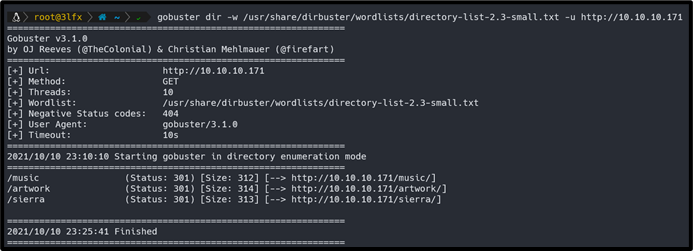
\includegraphics[width=0.99\textwidth]{imagenes/enudicopen.png}
    \caption{Enumeración de directorios en OpenAdmin}
\end{figure}
\par
Del proceso anterior se registró 3 directorios, se procedió a acceder al directorio music donde se encontraba la página SOLMUSIC.

\begin{figure}[H]
    \centering
    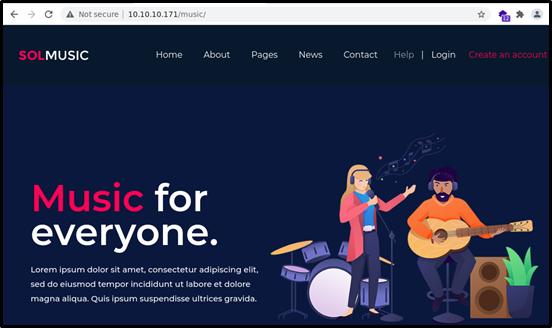
\includegraphics[width=0.99\textwidth]{imagenes/musicopen.png}
    \caption{Página web Music en OpenAdmin}
\end{figure}

Al revisar esta página se descubrió que al dirigirse al Login nos redirige al directorio “ona”. Se observa el uso del servicio OpenNetAdmin con versión 18.1.1 como se muestra en la siguiente imagen.

\begin{figure}[H]
    \centering
    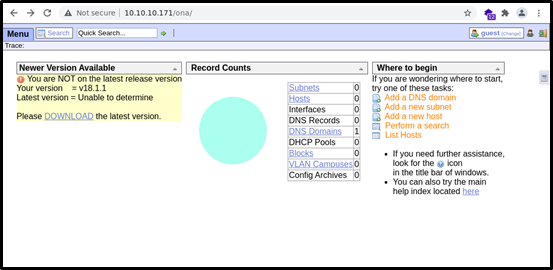
\includegraphics[width=0.99\textwidth]{imagenes/onaopen.png}
    \caption{Servicio OpenNetAdmin}
\end{figure}
Al buscar información sobre la versión de este servicio, se encontró que es vulnerable a ejecución remota de comandos (VU01).

La vulnerabilidad es debido a que la función “ws\_ping”, del módulo “tooltips”, realiza ejecución de código para realizar ping a una dirección IP, mediante el parámetro “form” donde se encontrará la IP esperada por la función utilizada, se puede inyectar comandos de Shell.
\subsubsection{Explotación}
Para la explotar la vulnerabilidad encontrada se utilizó un exploit escrito en Python perteneciente al usuario “amriunix” de GitHub \cite{ona}. Una vez descargado el exploit se ejecutó, obteniendo acceso a la máquina como “www-data”. 
\begin{figure}[H]
    \centering
    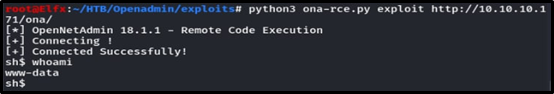
\includegraphics[width=0.99\textwidth]{imagenes/expopen.png}
    \caption{Ejecución de exploit en OpenAdmin}
\end{figure}
\subsubsection{Escalamiento de Privilegios}
Se procede a analizar los directorios con lectura permitida, encontrando el archivo “database\_settings.inc.php”, donde se encontró una contraseña en texto plano que resulta ser del usuario Jimmy (DE01).
\begin{figure}[H]
    \centering
    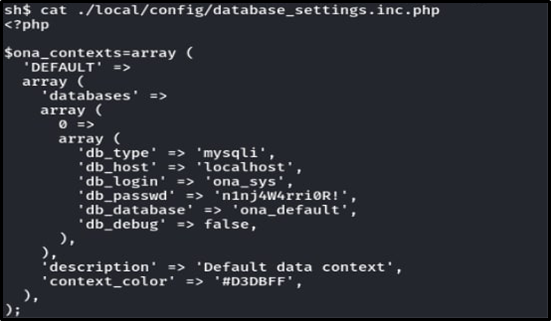
\includegraphics[width=0.8\textwidth]{imagenes/contsql.png}
    \caption{Hallazgo de contraseña en OpenAdmin}
\end{figure}
Una vez teniendo esta contraseña se procede a realizar una conexión mediante el servicio SSH como el usuario Jimmy, donde se consigue el acceso teniendo como prueba la siguiente imagen.
\par
\begin{figure}[H]
    \centering
    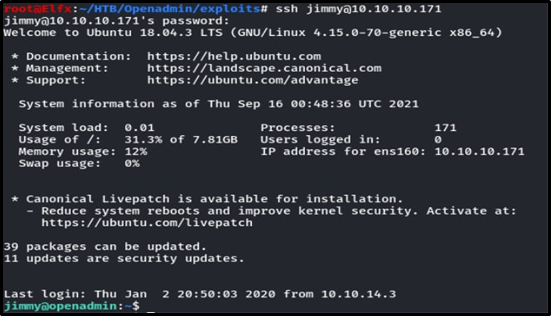
\includegraphics[width=0.8\textwidth]{imagenes/acjim.png}
    \caption{Acceso al usuario Jimmy en OpenAdmin}
\end{figure}

Lo siguiente a realizar es una búsqueda de archivos que nos permitan tener acceso al usuario Joanna. En el directorio “/var/www/internal” se encuentra el archivo “main.php” que al analizarlo se observa la ejecución de lectura del archivo “id\_rsa” perteneciente al usuario Joanna (DE02).
\begin{figure}[H]
    \centering
    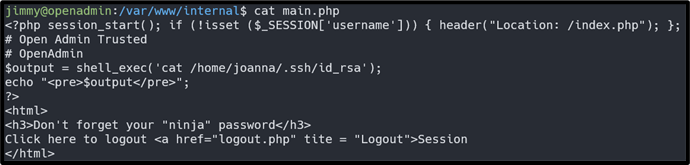
\includegraphics[width=0.99\textwidth]{imagenes/idjoa.png}
    \caption{Archivo de ejecución para lectura de ``id\_rsa" de Joanna}
\end{figure}
Para tener acceso a esta sección no se puede realizar mediante el puerto 80, por ello se revisa los puertos abiertos de la máquina desde adentro mediante netstat.
\begin{figure}[H]
    \centering
    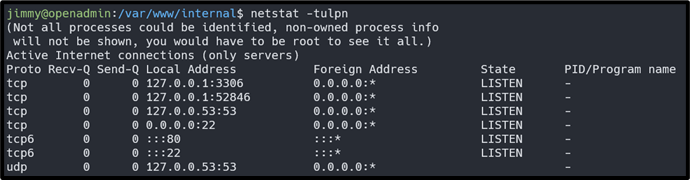
\includegraphics[width=0.99\textwidth]{imagenes/listpa.png}
    \caption{Listado de puertos abiertos internamente en OpenAdmin}
\end{figure}
Del proceso anterior se encuentra el puerto 3306 y 52846, teniendo éxito al realizar la llamada al archivo “main.php” a través del puerto 52846, como prueba de ello se tiene la siguiente imagen.
\begin{figure}[H]
    \centering
    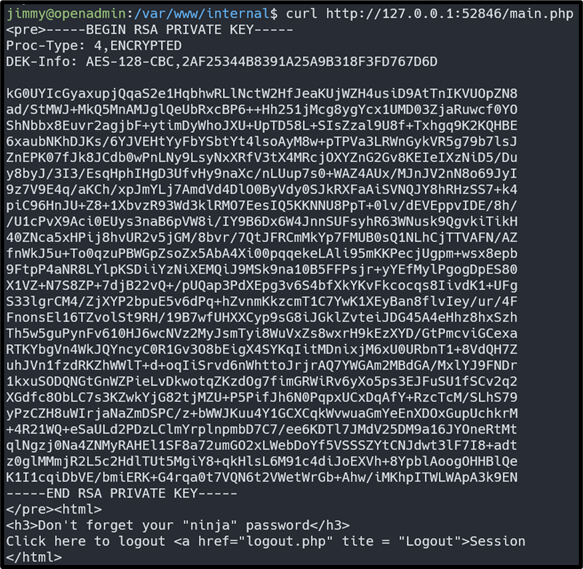
\includegraphics[width=0.58\textwidth]{imagenes/claprjoa.png}
    \caption{Clave privada de Joanna}
\end{figure}
Una vez obtenido la clave privada de Joanna que está protegida por una frase de contraseña como se indica en la imagen anterior, se procede a usar la herramienta “ssh2john” para convertir la clave privada en un hash que pueda ser descifrado con John the Ripper.
\begin{figure}[H]
    \centering
    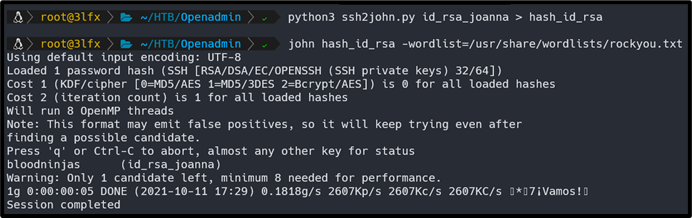
\includegraphics[width=0.99\textwidth]{imagenes/desjoa.png}
    \caption{Descifrado de contraseña de Joanna}
\end{figure}
Como resultado del descifrado se obtuvo que la frase de contraseña es “bloodninjas”. Ahora se puede realizar una conexión ssh a la máquina con el usuario Joanna, teniendo como prueba la siguiente imagen.
\begin{figure}[H]
    \centering
    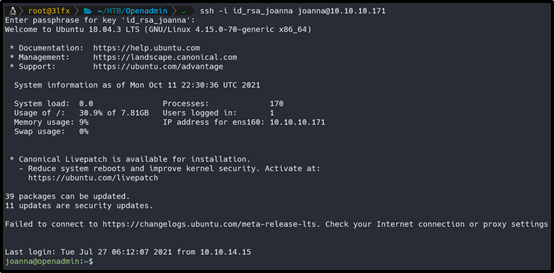
\includegraphics[width=0.99\textwidth]{imagenes/acjoa.png}
    \caption{Acceso al usuario Joanna en OpenAdmin}
\end{figure}
Una vez accedido al usuario Joanna se puede procederá a escalar privilegios a usuario “root”, para ello verificamos que comandos puede ejecutar en la máquina.
\begin{figure}[H]
    \centering
    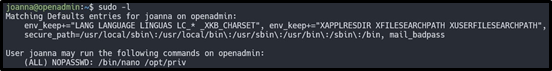
\includegraphics[width=0.99\textwidth]{imagenes/perejop.png}
    \caption{Permiso de ejecución sin contraseña con usuario Joanna}
\end{figure}
Como se muestra en la anterior imagen se puede ejecutar “/bin/nano /opt/priv” sin necesidad de contraseña, al proceder a ejecutarlo se abre nano con el archivo “/opt/priv”.
\begin{figure}[H]
    \centering
    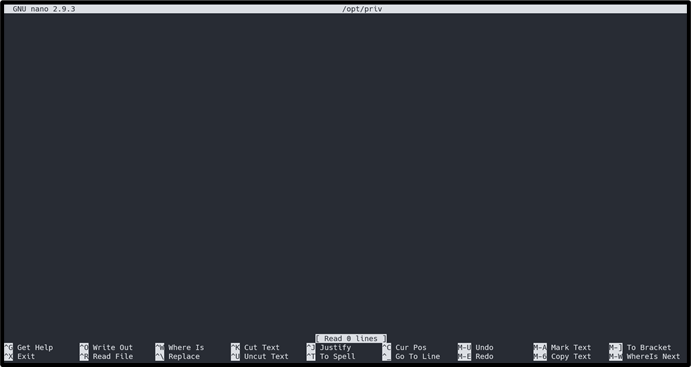
\includegraphics[width=0.99\textwidth]{imagenes/espop.png}
    \caption{Escalamiento de privilegios en OpenAdmin}
\end{figure}
Buscando información sobre escalamiento de privilegios mediante nano se encuentra que se puede obtener una Shell para ejecutar comandos como root utilizando la combinación de opciones “Ctrl+R” y “Ctrl+X” para ejecutar comando. El comando por ingresar será “reset; sh 1\textgreater\&0 2\textgreater\&0”, con el que se consigue una Shell.
\begin{figure}[H]
    \centering
    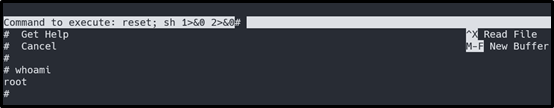
\includegraphics[width=0.99\textwidth]{imagenes/acroot.png}
    \caption{Acceso al usuario root en OpenAdmin}
\end{figure}
Una vez que se tiene la Shell, se procede a verificar que somos el usuario “root” como se indica en la imagen anterior.
\clearpage
\subsubsection{Post-explotación}
En la parte de post-explotación se procede a extraer los hashes pertenecientes a los usuarios del sistema.
\begin{figure}[H]
    \centering
    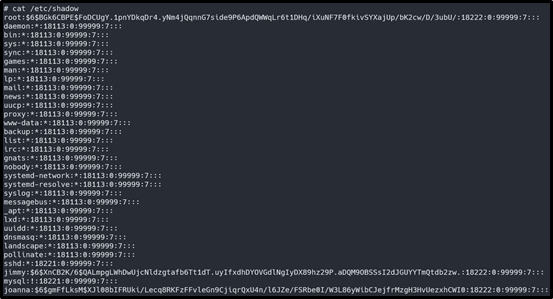
\includegraphics[width=0.99\textwidth]{imagenes/hashop.png}
    \caption{Contraseñas en formato hash de OpenAdmin}
\end{figure}
\subsubsection{Recomendaciones de mitigación}
Las recomendaciones para evitar ataques mediante las vulnerabilidades y debilidades encontradas en la maquina OpenAdmin son las siguientes.
\begin{itemize}
    \item Cambiar el uso del Software OpenAdmin a uno con mayor frecuencia de actualizaciones, debido a que la versión usada en esta máquina es la última, y no recibe actualizaciones desde junio del 2018.
    \item Realizar un control en cuanto a los permisos de ejecución privilegiados permitidos a un usuario y que pueda ocasionar el escalamiento de privilegios en el sistema.
\end{itemize}
    \subsection{HTB02 - Magic}
\subsubsection{Escaneo}
En la fase de escaneo mediante la herramienta “Nmap” se observó que se encontraban 2 puertos abiertos, el puerto 22 del servicio SSH y el puerto 80 usando como servidor Apache.
\begin{figure}[H]
    \centering
    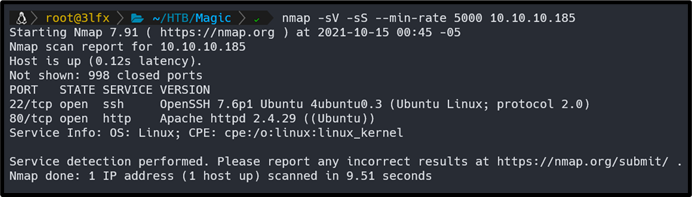
\includegraphics[width=0.99\textwidth]{imagenes/scanmag.png}
    \caption{Escaneo de puertos Magic}
\end{figure}
\subsubsection{Análisis de Vulnerabilidades y debilidades}
Se procedió a analizar el sitio web de la máquina, teniendo vista de varias imágenes.
\begin{figure}[H]
    \centering
    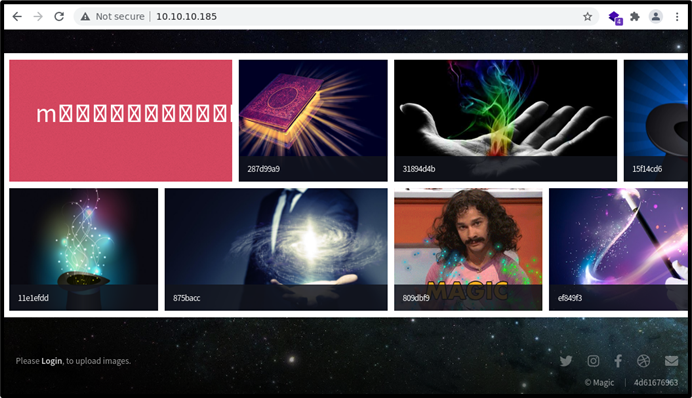
\includegraphics[width=0.99\textwidth]{imagenes/pagmag.png}
    \caption{Página web Magic}
\end{figure}
En la parte de abajo se observa que se necesita iniciar sesión para subir imágenes. Por ello se procede a dirigirse al Login teniendo el siguiente formulario.
\begin{figure}[H]
    \centering
    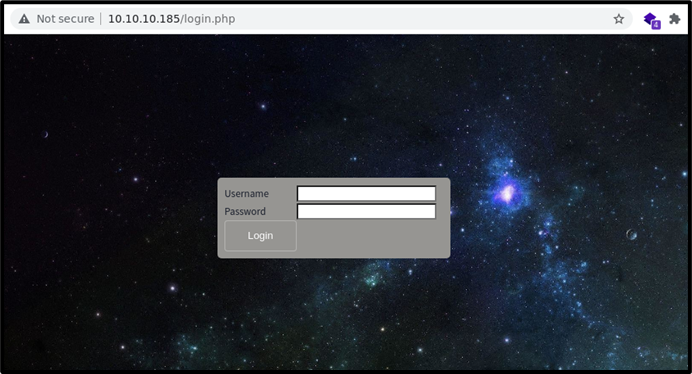
\includegraphics[width=0.9\textwidth]{imagenes/logmag.png}
    \caption{Servicio Login en sitio web Magic}
\end{figure}
Se intentó algunos usuarios y contraseñas genéricas sin tener éxito donde se notificaba que el usuario o contraseña era incorrecto, lo siguiente a realizar fue intentar una inyección SQL teniendo como parámetro de username (’ 1=1;) y en la contraseña cualquier valor, después de ello se recarga la página, pero sin indicarnos que el usuario o contraseña era incorrecto, lo que indica que si es vulnerable a inyección SQL (VU02, DE03). Continuando con la inyección SQL se realizó utilizando para acceder al usuario “admin” al usar como parámetro de username (admin’;), esto permite acceder a la página de “upload.php” como se puede ver en la siguiente imagen.
\begin{figure}[H]
    \centering
    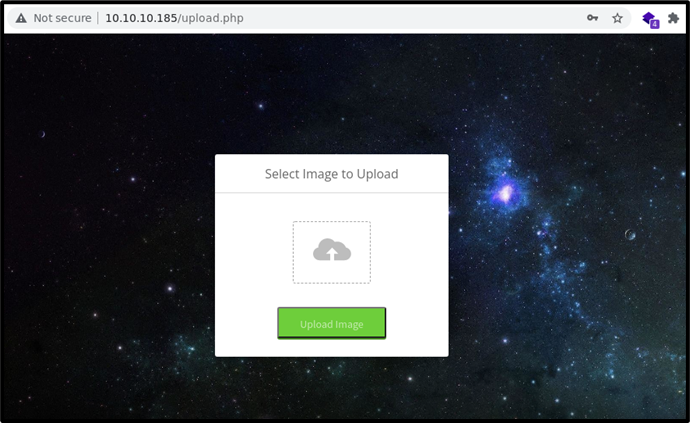
\includegraphics[width=0.9\textwidth]{imagenes/submag.png}
    \caption{Página para subida de imágenes en Magic}
\end{figure}
\subsubsection{Explotación}
Una vez teniendo acceso para subir imágenes, se procede a la fase de explotación donde al tener permitido el subido de archivos, se procederá a tener acceso mediante una Reverse Shell. Se intentó subir un archivo con la terminación “.php”, pero no permite otros archivos que no sean imágenes, también se hizo la prueba cambiándole la extensión, pero el servidor valida los metadatos para confirmar que sean imágenes (DE04).

Por ello se incrusto una carga útil a una imagen real para realizar la Reverse Shell, esto se hizo con la herramienta “exiftool” agregando la carga útil en como comentario de la imagen y se cambió la extensión a “.php.jpg”.
\begin{figure}[H]
    \centering
    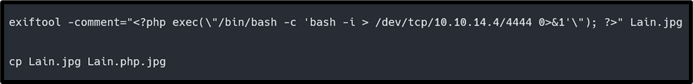
\includegraphics[width=0.99\textwidth]{imagenes/inyima.png}
    \caption{Inyección de código malicioso en imagen}
\end{figure}
Se procede subiendo el archivo y es aceptado por el servidor, ahora se consulta la imagen en la ruta “/images/uploads/” donde estaban todas las demás imágenes que aparecen en la página principal. Esto genera el acceso a la máquina como “www-data” como se puede apreciar en la siguiente imagen.
\begin{figure}[H]
    \centering
    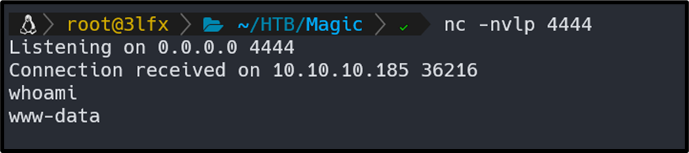
\includegraphics[width=0.8\textwidth]{imagenes/acwma.png}
    \caption{Acceso como ``www-data” en máquina Magic}
\end{figure}
\subsubsection{Escalamiento de Privilegios}
Para el escalamiento de privilegios se revisó el directorio “Magic”, abriendo el archivo “db.php5” donde se encontró un usuario y contraseña de base de datos como se muestra en la siguiente imagen (DE01).
\begin{figure}[H]
    \centering
    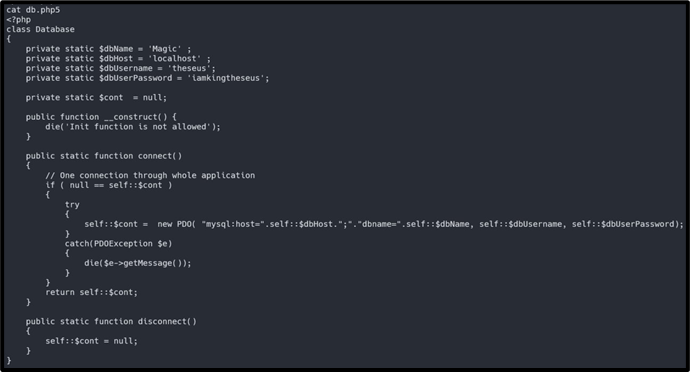
\includegraphics[width=0.99\textwidth]{imagenes/conarma.png}
    \caption{Contraseña en archivo de configuración en máquina Magic}
\end{figure}
Se intentó acceder a la máquina como “Theseus” con esa contraseña, pero no se tuvo éxito, por ello se intenta usar el comando “mysql” pero no existe, luego buscando otro comando para ejecutar se intentó “mysqldump” para extraer la información de la base de datos.
\begin{figure}[H]
    \centering
    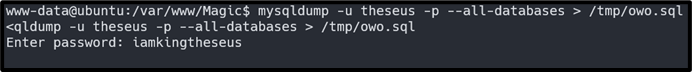
\includegraphics[width=0.99\textwidth]{imagenes/basemag.png}
    \caption{Extracción de tablas de base de datos en Magic}
\end{figure}
Una vez realizado el proceso anterior, se procede a leer el archivo generado, encontrando allí otra contraseña como se muestra en la siguiente imagen.
\begin{figure}[H]
    \centering
    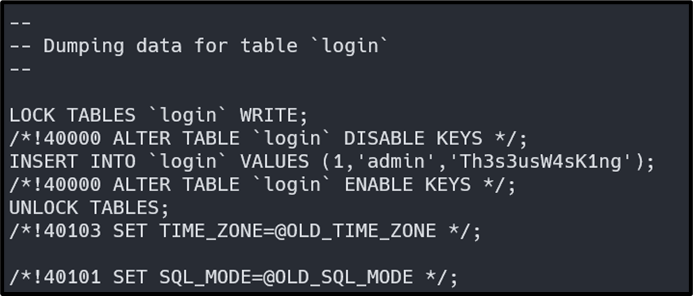
\includegraphics[width=0.9\textwidth]{imagenes/tabmag.png}
    \caption{Contraseña en base de datos Magic}
\end{figure}
Con esa contraseña encontrada se procede a intentar acceder mediante el usuario Theseus y se consigue exitosamente, como prueba se tiene la siguiente imagen.
\begin{figure}[H]
    \centering
    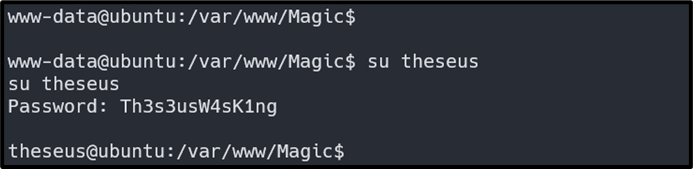
\includegraphics[width=0.99\textwidth]{imagenes/acthe.png}
    \caption{Acceso a usuario Theseus en Magic}
\end{figure}
Se procede a listar los archivos con permiso SUID mostrando esta lista en la siguiente imagen.
\begin{figure}[H]
    \centering
    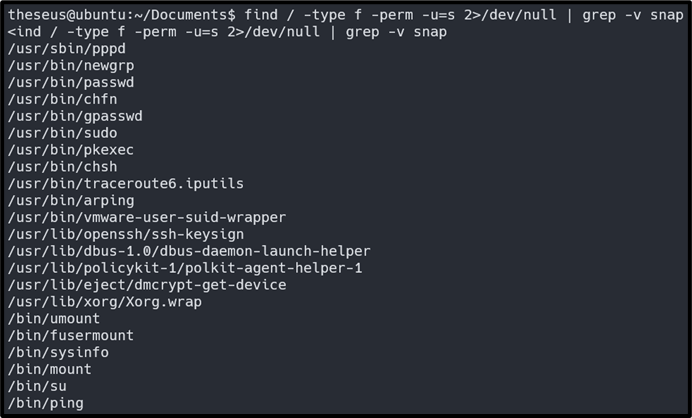
\includegraphics[width=0.99\textwidth]{imagenes/listsuma.png}
    \caption{Listado de archivos con permiso SUID en Magic}
\end{figure}
Del proceso anterior se observa el archivo “sysinfo” del que se procederá a analizar su función. A partir de los caracteres imprimibles se encuentra que ejecuta ciertos comandos .
\begin{figure}[H]
    \centering
    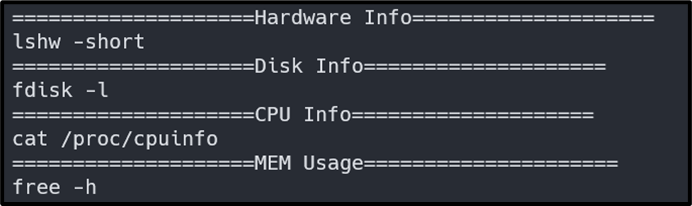
\includegraphics[width=0.9\textwidth]{imagenes/sysin.png}
    \caption{Comandos que ejecuta ``sysinfo''}
\end{figure}
Se encontró información de este programa que cuenta con una vulnerabilidad, por ello se procederá a realizar un secuestro de PATH para escalar privilegios (VU03, DE07).

Lo siguiente a realizar es crear un archivo “lshw” con la que se obtendrá una Reverse Shell, y pasar el archivo desde la máquina atacante hacia la victima mediante el levantamiento de un servidor HTTP con Python.
\begin{figure}[H]
    \centering
    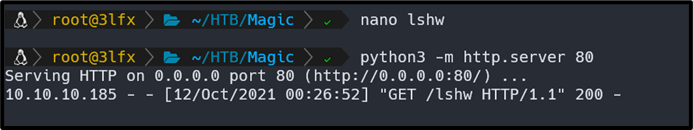
\includegraphics[width=0.9\textwidth]{imagenes/seratma.png}
    \caption{Servidor HTTP en máquina atacante}
\end{figure}
En la máquina víctima se procede a descargar el archivo creado y se le cambia los permisos de ejecución para luego proceder a agregar el directorio “/tmp” al PATH lo que permitirá la ejecución de archivo creado mediante el binario “sysinfo”.
\begin{figure}[H]
    \centering
    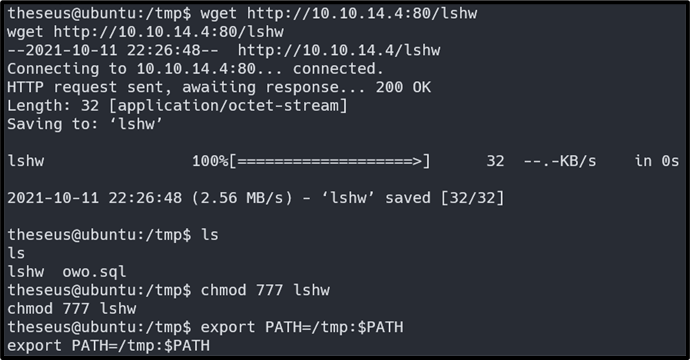
\includegraphics[width=0.9\textwidth]{imagenes/armalmag.png}
    \caption{Configuración de archivo malicioso en Magic}
\end{figure}
Lo siguiente a realizar tener en escucha el puerto indicado en el archivo “lshw” y después ejecutar el comando “sysinfo”, como resultado se obtiene conexión a la máquina objetivo como el usuario “root”.
\begin{figure}[H]
    \centering
    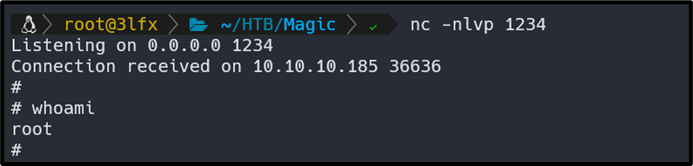
\includegraphics[width=0.9\textwidth]{imagenes/acrootmag.png}
    \caption{Acceso al usuario root en máquina Magic}
\end{figure}
\subsubsection{Post-explotación}
En la fase de post-explotación se procede a extraer las credenciales de los usuarios pertenecientes a la máquina “Magic”, teniendo de prueba la siguiente imagen.
\begin{figure}[H]
    \centering
    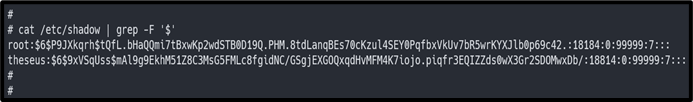
\includegraphics[width=0.99\textwidth]{imagenes/hashmag.png}
    \caption{Extracción de contraseñas en formato hash de Magic}
\end{figure}
\subsubsection{Recomendaciones de mitigación}
Para mitigar las vulnerabilidades y debilidades encontradas en la máquina Magic, se recomienda lo siguiente:
\begin{itemize}
    \item Neutralizar correctamente los elementos especiales al momento de realizar comandos SQL en el servicio Login, con la finalidad de evitar el acceso no autorizado mediante la inyección SQL en el sitio web.
    \item Realizar un mejor control de archivos permitidos para cargar al sitio web para evitar que se suba imágenes con código malicioso que permita el acceso al sistema.
    \item No utilizar herramientas como “sysinfo”, que se ejecutan con altos privilegios, lo que permitiría a un usuario el escalamiento de privilegios, o en su defecto configurarlo para que solo se permita su ejecución por el usuario “root”.
\end{itemize}
    \subsection{HTB03 - Remote}
\subsubsection{Escaneo}
\subsubsection{Análisis de Vulnerabilidades y debilidades}
\subsubsection{Explotación}
\subsubsection{Escalamiento de Privilegios}
\subsubsection{Post-explotación}
\subsubsection{Recomendaciones de mitigación}
    \subsection{HTB04 - Fuse}
\subsubsection{Escaneo}
\subsubsection{Análisis de Vulnerabilidades y debilidades}
\subsubsection{Explotación}
\subsubsection{Escalamiento de Privilegios}
\subsubsection{Post-explotación}
\subsubsection{Recomendaciones de mitigación}
\clearpage
%---conclusiones----
\addcontentsline{toc}{section}{Conclusiones}%--para añadir seccion a las conclusiones
\begin{center}
    \section*{Conclusiones}
\end{center}
El equipo auditor concluye de la presente evaluación de penetración de seguridad lo siguiente:
\begin{itemize}
    \item En los cuatro computadores se encontraron vulnerabilidades o debilidades graves que permitieron el acceso como superusuario o administrador.
    \item Dentro de las vulnerabilidades encontradas el 40\% son del tipo Ejecución Remota de Código.
    \item El porcentaje de máquinas que tienen como debilidad la exposición de información confidencial a un actor no autorizado es de 75\%.
    \item Para los cuatro casos se registraron las vulnerabilidades halladas, métodos de explotación, evidencias de post-explotación y recomendaciones de mitigación.
    \item Los riesgos que se pueden presentar para los casos mencionados son el robo de información sensible, alteración de servicios web y control de los sistemas.
\end{itemize}
\clearpage
%---recomendaciones--
\addcontentsline{toc}{section}{Recomendaciones}%--para añadir seccion a las conclusiones
\begin{center}
    \section*{Recomendaciones}
\end{center}
Las recomendaciones para resolver las vulnerabilidades halladas y evitar daños futuros son las siguientes:
\begin{itemize}
    \item Actualizar con frecuencia la versión de los diferentes programas y servicios usados por las computadoras.
    \item Usar de preferencia software con soporte continuo para evitar ataques cuando se reportan vulnerabilidades.
    \item Realizar controles sobre la información confidencial expuesta hacia actores no autorizados.
    \item No guardar contraseñas en archivos de configuración de los servicios ofrecidos.
    \item Neutralizar correctamente los elementos especiales en comandos SQL.
    \item Realizar un control estricto sobre los requisitos de las contraseñas para evitar contraseñas débiles ante fuerza bruta.
    \item Verificar los permisos habilitados sobre los usuarios que podrían permitir el escalamiento de privilegios no deseados.
    \item Prevenir que los programas con altos privilegios realicen ejecución mediante rutas relativas y no rutas absolutas.
    \item Realizar un control sobre los archivos permitidos a subir, para evitar archivos maliciosos.
    \item No usar servicios sin autenticación para compartir información confidencial.
\end{itemize}
%--referencias
\clearpage

\addcontentsline{toc}{section}{Referencias}
\begin{thebibliography}{0}
    \bibitem{cvedetails} CVE security vulnerability database. Security vulnerabilities, exploits, references and more. CVE Details. \href{https://www.cvedetails.com}{https://www.cvedetails.com}
    \bibitem{vulmon} Vulmon - Vulnerability Intelligence Search Engine. Vulmon. \href{https://vulmon.com}{https://vulmon.com}
    \bibitem{cwe} MITRE. CWE - Common Weakness Enumeration. CWE. \href{https://cwe.mitre.org}{https://cwe.mitre.org}
    \bibitem{ona} GitHub - amriunix/ona-rce: OpenNetAdmin 18.1.1 - Remote Code Execution. GitHub. \href{https://github.com/amriunix/ona-rce}{https://github.com/amriunix/ona-rce}
    \bibitem{crack} CrackStation - Online Password Hash Cracking - MD5, SHA1, Linux, Rainbow Tables, etc. CrackStation. \href{https://crackstation.net/}{https://crackstation.net/}
    \bibitem{umbraco} GitHub - noraj/Umbraco-RCE: Umbraco CMS 7.12.4 - (Authenticated) Remote Code Execution. GitHub. \href{https://github.com/noraj/Umbraco-RCE}{https://github.com/noraj/Umbraco-RCE}
    \bibitem{invokepower} nishang/Invoke-PowerShellTcp.ps1 at master · samratashok/nishang. GitHub. \href{https://github.com/samratashok/nishang/blob/master/Shells/Invoke-PowerShellTcp.ps1}{https://github.com/samratashok/nishang/blob/master/Shells/Invoke-PowerShellTcp.ps1}
    \bibitem{powerup} PowerSploit/PowerUp.ps1 at master · PowerShellMafia/PowerSploit. GitHub. \href{https://github.com/PowerShellMafia/PowerSploit/blob/master/Privesc/PowerUp.ps1}{https://github.com/PowerShellMafia/PowerSploit/blob/master/Privesc/PowerUp.ps1}
    \bibitem{roguewin} GitHub - antonioCoco/RogueWinRM: Windows Local Privilege Escalation from Service Account to System. GitHub. \href{https://github.com/antonioCoco/RogueWinRM}{https://github.com/antonioCoco/RogueWinRM}
    \bibitem{mimikatz} GitHub - ParrotSec/mimikatz. GitHub. \href{https://github.com/ParrotSec/mimikatz}{https://github.com/ParrotSec/mimikatz}
    \bibitem{evilwinrm} GitHub - Hackplayers/evil-winrm: The ultimate WinRM shell for hacking/pentesting. GitHub. \href{https://github.com/Hackplayers/evil-winrm}{https://github.com/Hackplayers/evil-winrm}
    \bibitem{exploitcapcom} GitHub - tandasat/ExploitCapcom: This is a standalone exploit for a vulnerable feature in Capcom.sys. GitHub. \href{https://github.com/tandasat/ExploitCapcom}{https://github.com/tandasat/ExploitCapcom}
    \bibitem{loaddriver} GitHub - TarlogicSecurity/EoPLoadDriver: Proof of concept for abusing SeLoadDriverPrivilege (Privilege Escalation in Windows). GitHub. \href{https://github.com/TarlogicSecurity/EoPLoadDriver/}{https://github.com/TarlogicSecurity/EoPLoadDriver/}
\end{thebibliography}

\end{document}